\documentclass[letterpaper, 12pt, oneside]{book}
\usepackage[margin = 1in, includehead, footskip=0.25in]{geometry}
\usepackage{setspace}
\doublespacing
\usepackage{amsfonts}
\usepackage{amsmath}
\usepackage{amsthm}
\usepackage{tikz}
\usepackage{graphicx}
\usepackage{multirow}
\usepackage{booktabs}
\usepackage{tabularx}
\usepackage{longtable}
\usepackage{lscape}
\usepackage{import}
\usepackage[style=phys]{biblatex}
\bibliography{thesis_refs}
%\addbibresource{thesis_refs.bib}
\usepackage{lineno}
\linenumbers
\usepackage[pdfauthor={My Full Name},
    pdftitle={Title},
    hidelinks
]{hyperref}
\newtheorem{lemma}{Lemma}[section]
\theoremstyle{definition}
\newtheorem{definition}{Definition}[section]
\newtheorem{corolary}{Corolary}[section]
%\author{Skadi K Grossberndt}
%\title{Energy Correlators as a probe of the hard process in Run 24 $p-p$ collisions at $\sqrt{s}=200$ $GeV$ with the sPHENIX detector at RHIC}
%\affil{Graduate Center and Baruch College, CUNY}
\begin{document}
%\maketitle
\frontmatter
\begin{titlepage}

\begin{center}

~\vspace{2in}

\textsc{Energy Correlators as a probe of the hard process in Run 24 $p-p$ collisions at $\sqrt{s}=200$ $GeV$ with the sPHENIX detector at RHIC} \\[0.5in]
by \\[0.5in]
\textsc{Skadi Kurt Grossberndt} 

\vspace{\fill}
A dissertation submitted to the Graduate Faculty in Physics in partial fulfillment of the requirements for the degree of Doctor of Philosophy, The City University of New York \\[0.25in]
2025

\end{center}

\end{titlepage}

\setcounter{page}{2}
\phantom{}\vspace{\fill}
\begin{center}
\copyright~2025\\
\textsc{Skadi Kurt Grossberndt}\\
All Rights Reserved\\
\end{center}

\begin{center}
This manuscript has been read and accepted by the Graduate Faculty in Physics in satisfaction of the dissertation requirement for the degree of Doctor of Philosophy.
\end{center}

\vspace{0.75in}

\begin{tabular}{p{1.75in}p{0.5in}p{3.5in}}
~                                   & & \textbf{Professor Stefan Bathe}\\
~                                   & & \\
\hrulefill                          & &\hrulefill \\
Date                                & & Chair of Examining Committee\\
~                                   & & \\
~                                   & & \textbf{Professor Tom Jones}\\
~                                   & & \\
\hrulefill                          & &\hrulefill \\
Date                                & & Executive Officer\\
\end{tabular}

\vspace{0.75in}

\begin{tabular}{l}
\textbf{Professor Adrian Dimitru} \\
\textbf{Professor Raghav K} \\
\textbf{Professor Jamal Jallian-Marian} \\
\textbf{Professor Z} \\
Supervisory Committee \\
\end{tabular}


\vspace{\fill}
\begin{center}
\textsc{The City University of New York}
\end{center}

\begin{center}
Abstract \\
\textsc{Energy Correlators as a probe of the hard process in Run 24 $p-p$ collisions at $\sqrt{s}=200$ $GeV$ with the sPHENIX detector at RHIC} \\
by \\
\textsc{Skadi K Grossberndt} \\[0.25in]
\end{center}

\vspace{0.25in}

\noindent Adviser: Professor Stefan Bathe

\vspace{0.25in}

\noindent This dissertation consists of three parts in addition to a literature review establishing the state of the art of jet physics and the Energy-Energy correlator at high energies\ldots

\paragraph{Part 1: Hardware} %\input{One.tex}
This part discusses the physical hardware used to make the measurements of the energy in the jets created by the proton-proton collisions. 
This part contains a discussion of the sPHENIX detector and an in-depth look at the relevant susbsystems for the meausements in this analysis. 
In addition, the Monte Carlo methods and models to discern the expected respnse and calibrate the detector are discussed in detail, with both subparts coming together in a disucssion of backgrounds and error calculation in general and for the observables at hand.
\paragraph{Part 2: Technicalities} %\input{Two.tex}
This part builds from first principles up to the jet measurement in a theoretical light, and then discusses the additional computational techniques on display that will provide the bridge between the theory of these observables and the practical application to sPHENIX. 
This part continains a chapter that is a pared down discussion of a midstream paper proposed as part of the thesis process that establishes the safety of this observable against jet finding choices.
\paragraph{Part 3: Experimental Output} %\input{Three.tex}
This part is the meet and potatoes of the dissertation, discussing results from the experiment and the analysis in light of the previous parts and comparing to the world results from related systems.


\include{Acknowledgements}

\tableofcontents
\listoftables
\listoffigures

\mainmatter
\chapter{Literature Review}
\label{ch:LR}
%\documenclass[Skadi_Thesis_Draft.tex]{subfiles}
%\begin{document}
\section{Jets Definitions}
The study of Quantum Chromodynamics in high energy collisions, such as those at the Relativistic Heavy Ion Collider or the Large Hadron Collider, is often carried out through investigation of the kinematics of jets.
Jets, as objects, sit in the boundary between experiment and theory, being an experimental signature corresponding to final states of quarks and gluons produced in collisions. 
Jets are a cluster of final state particles that result from the showering and hadronization of the initial parton, that are identified in experiment through use of one of the multiple jet reconstruction algorithms. 
\subsection{Jet Reconstruction Algorithms}
In Ryan Atkin's paper \textit{Review of jet reconstruction algorithms} \cite{Atkin2015}, Atkin provides an overview of the standard algorithms with a focus on practical implementation for experimental usage. %this is a very basic conference note style papaer, should probably just use it as an intro to each method
Atkin discusses a number of algorithms that fall into two categories: Cone based and Sequential Clustering 
\subsubsection{Cone Methods}
	In Atkin's paper, Atkin discusses two iterative cone procedures--Iterative Cone with Progressive Removal and with Split Merge--and one more modern cone method, Seedless Infrared Safe Cone. 
	These iterative cone procedures are described as simple to implement in an experimental context, however, they both suffer deficiencies from a theoretical perspective as they fail to be IRC safe \cite{Atkin2015} \cite{Salam2007}.

\subsection{Quark and Gluon Jets}	
	In their paper \textit{An Operational Definition of Quark and Gluon Jets} \cite{Komiske2018} Kimiske, Metodiev and Thaler present a theoretical definition of jet flavor with an eye towards application at colliders. 
	They aim to present a precise and practical definition of jet flavor at the hadron level, thus allowing for direct measurement from collider experiments rather than a measurement by proxy. 
	While the gluon or quark jet is well defined at the level of the hard scattering, corresponding to an initiating parton of the primary vertex \cite{Jones1989} \cite{Fodor1990}. 
	Experimentally, there is significant interest in being able to discriminate quark and gluon jets in searches for Beyond Standard Model physics, searches for Dark Matter, in jet substructure analysis and in QGP physics. \cite{Gallicchio2011}\cite{Lima2017}\cite{Bhattacherjee2017}\cite{}. 
	The determination of relative populations of quark and gluon jets in a dijet sample is one of the primary tasks of this thesis and will be discussed at length in chapters \ref{ch:alphas} and \ref{ch:qgdiscr}. 

	Kimiske et al.--from here referred to as KMT--set their work in the context of discerning the quark-gluon jet populations in samples rather than applying an event-by-event labeling scheme. 
	KMT's work 
\section{Jet Substructure Measurements}

\section{N-Point Energy Correlator}
%\end{document}
 
\part{Hardware: The Detector and Simulations}
\chapter{The sPHENIX detector}
The sPHENIX detector is part of the Relativistic Heavy Ion Collider (RHIC) complex at Brookhaven National Laboratories (BNL) in Upton, New York. 
RHIC is one of two major circlular particle colliders in the world, the other of which is the Large Hadron Collider at CERN in Geneva, Switzerland. 
Over the course of the sPHENIX experiment which will run from run 23 until RHIC ceases opperations after run 25, RHIC will be colliding gold nuclei and protons with run 23 having been dedicated to commissioning Au+Au running, 
run 24 dedicated to p+p with three weeks of Au+Au for further tracking commisioning and run 25 dedicated to physics running in Au+Au collisions. 
RHIC runs with a center of mass energy of $\sqrt{s} = 200 GeV$ for both protons and gold, and additionally is the sole collider that collides polarized protons, which allows for more in depth studies of spin physics. 
At RHIC, sPHENIX's forerunner, the Pioneering High Energy Nuclear Interaction eXperiment (PHENIX), perfomed the first measurement of the Quark Gluon Plasma droplets \cite{QGP_droplets} in nuclei-nuclei collisions. 

sPHENIX is designed to offer significant upgrades to PHENIX, specifically provinding increased coverage with hadronic and electromagnetic calorimeters, increasing effectiveness in studies of jets and heavy flavor at mid-to-high Bjorken x \cite{sPHENIX_TDR}\cite{sPHENIX_whitepaper}\cite{sPHENIX_physics_goals}
Broadly, sPHENIX can be broken into three categories of subystem: Calorimerters, Tracking and Event characterization.
sPHENIX is constructed around a 4 Tesla superconducting magnet, cooled by liquid helium, which was previously used on the BABAR experiment at SLAC. 
\begin{figure}
	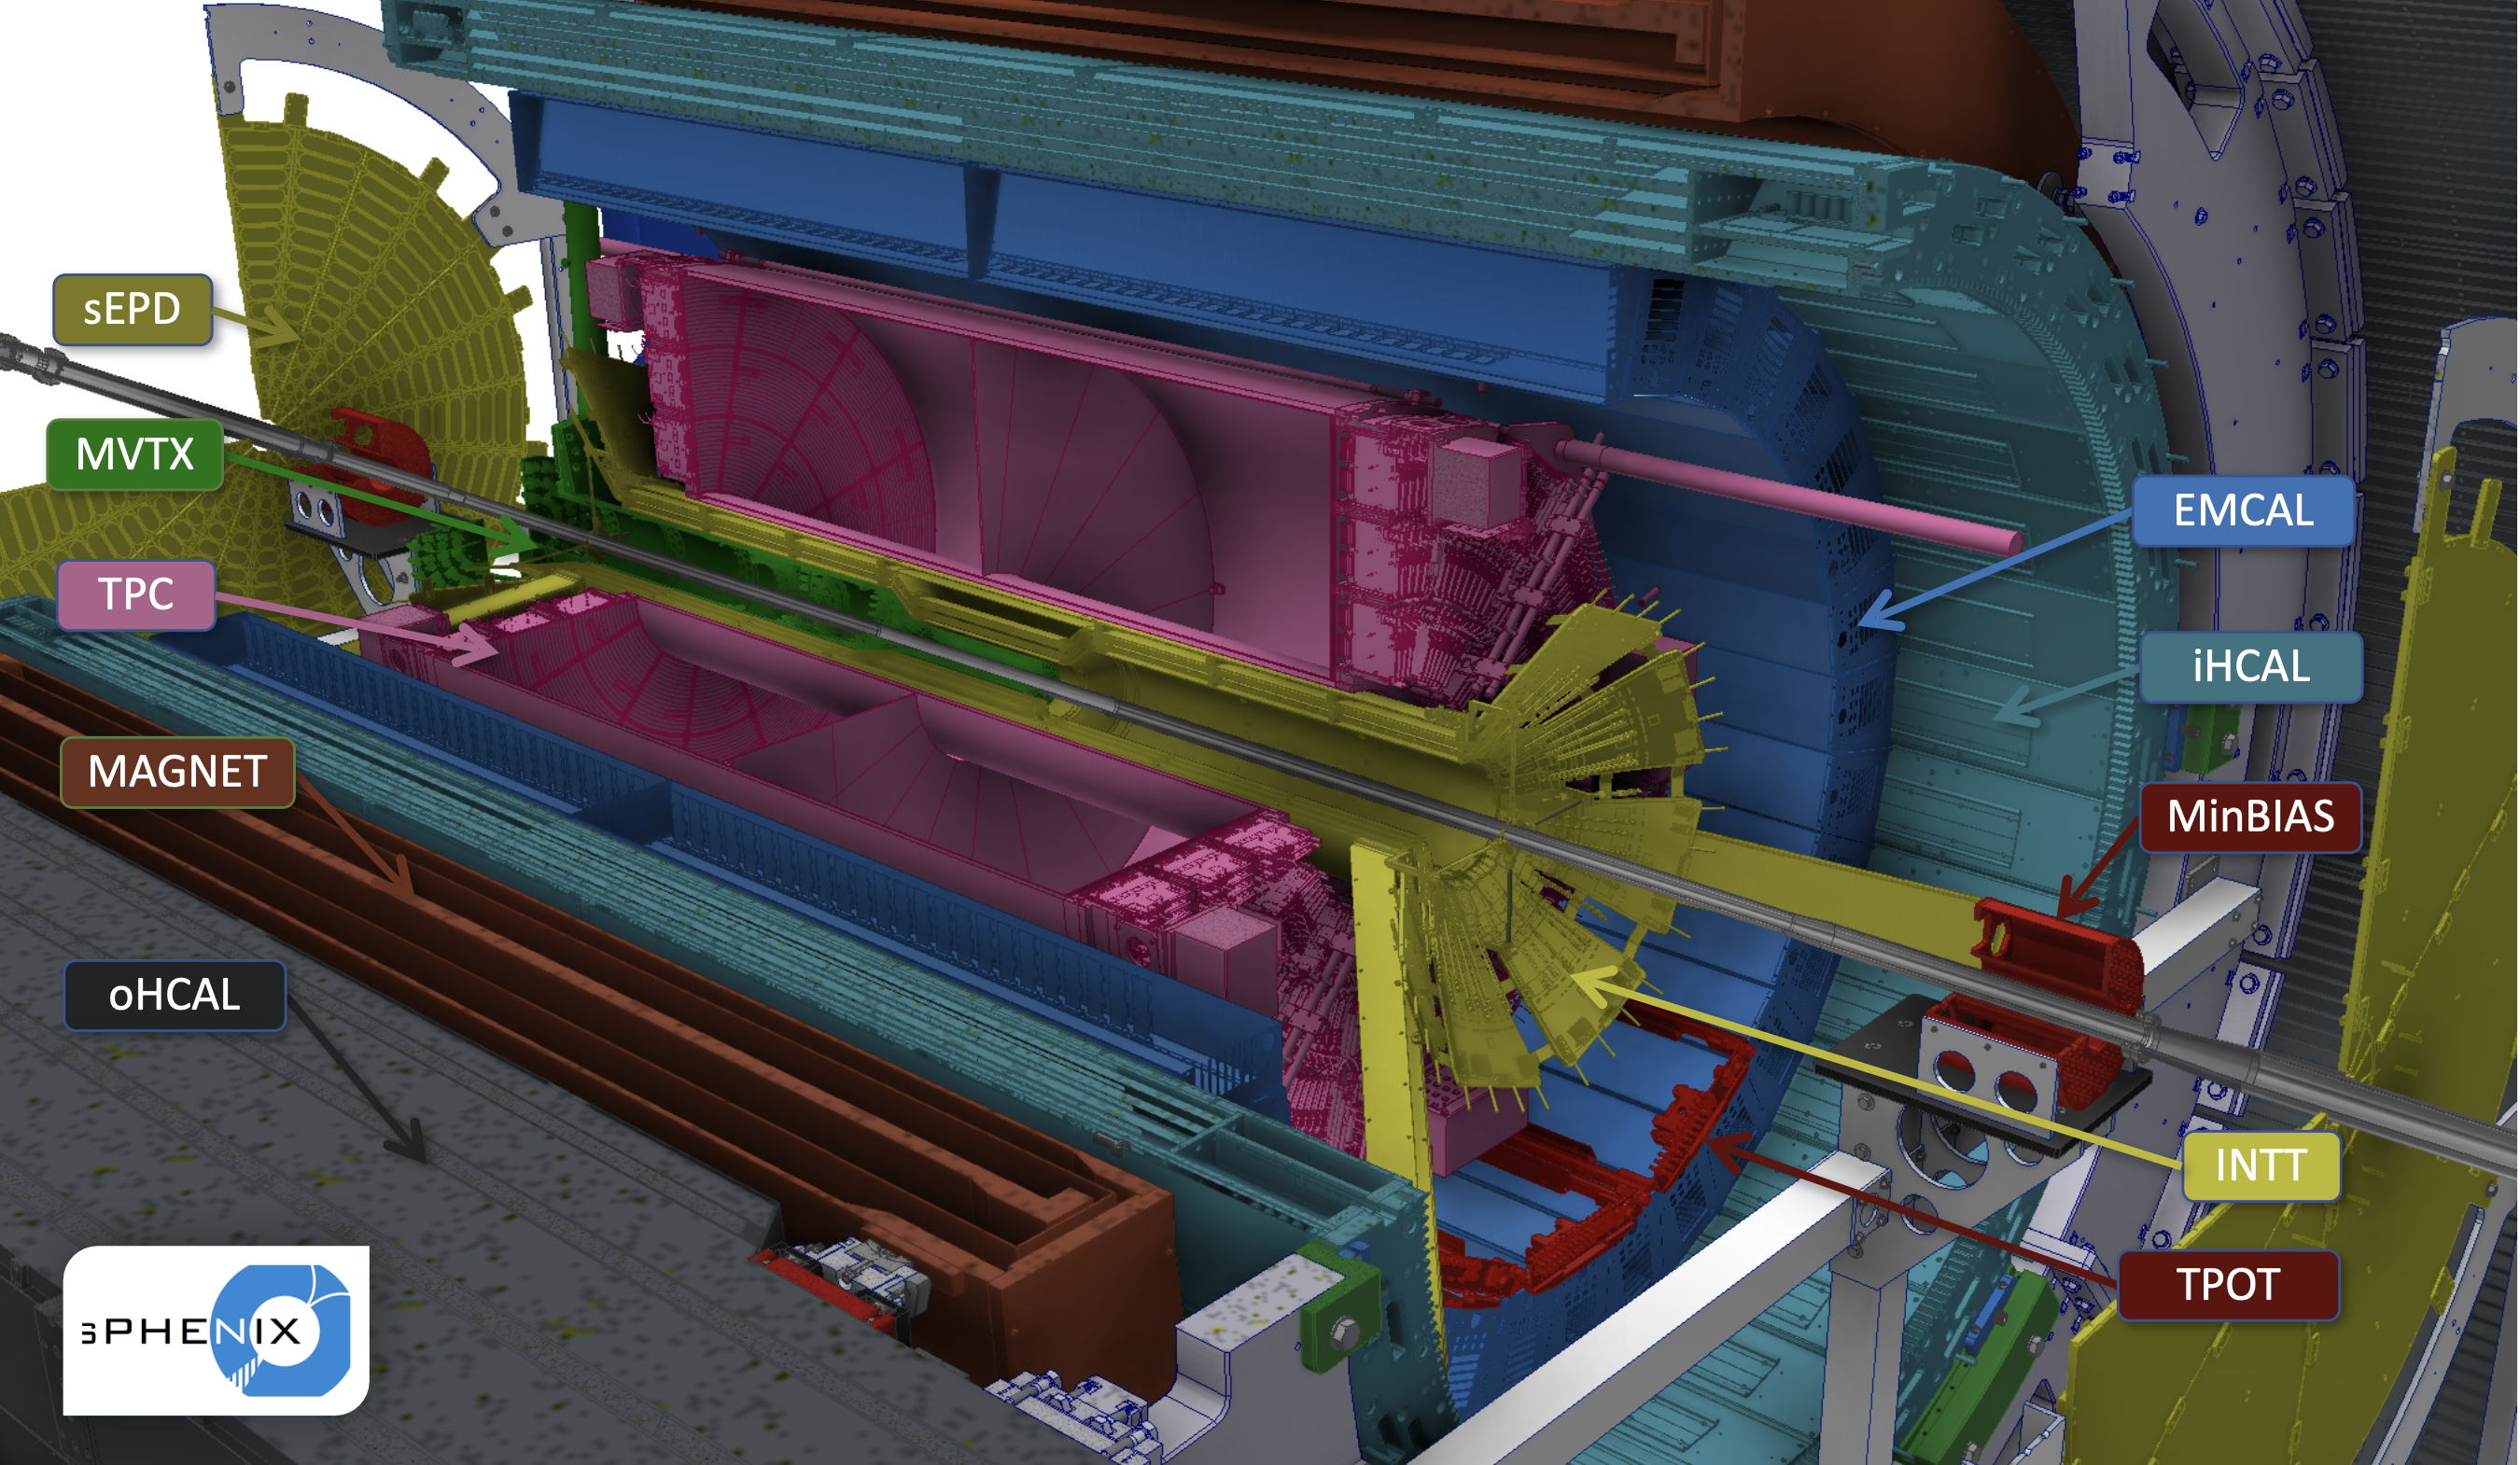
\includegraphics[scale=0.5]{sphenix_detector}
	\caption{The sPHENIX detector. The Zero Degree Calorimeter is not picutred but is located further along the beam pipe.}
	\label{fig:sphenix_detector}
\end{figure}
\section{Calorimetery}
	\subsection{Hadronic Calorimeters}
		sPHENIX's power in jet physics comes in large part from its calorimeter systems, including two seperate hadronic calorimeters. 
		The outer and inner hadronic calorimeter (OHCal and IHCal respectively) are both divided into 24 bins in $\eta$ with coverage of $|\eta| \leq 1.1$  and full $\varphi$ coverage with 64 bins in $\varphi$, grouped in $\varphi$ into 32 sectors in each calorimeter. 
		Each hadronic calorimeter therefore has tower size of $\delta \eta = 0.092$ and $\delta \varphi=0.098$.  
		The outer hadronic calorimeter is constructed of steel and sits outside of the magnet, with inner radius of $r=$ m and outer radius of $r=$ m. 
		The inner hadronic calormeter is constructed of aluminum and sits just inside the magnet, with inner radus of $r=$ m and outer radius of $r=$ m. 
		Each tower corresponds to a readout board that sums readout from four scintillator paddles embeded into the calorimeter as show in fig. \ref{fig:hcal}. 
		These interface boards form a single readout channel, and can be indvidually teste via a pulser system that injects charge into the interface board testing readback independent of scintillator response, and LED system that injects a fixed pulse of light into the scintilators to test behavior of the Silicon Photomultipliers (SiPMs). 
		Output of each of these systems is shown in fig \ref{fig:hcal_tests}
		\begin{figure}
			%need to figure out how to do the subfigures for this 
			\includegraphics{ihcal_pulser}
			\includegraphics{ohcal_pulser}
			\includegraphics{ihcal_led}
			\includegraphics{ohcal_led}
			\caption{Figuring out the subfigs first. But Left Pulser and Right LED, top IHCAL both OHCAL}
			\label{fig:hcal_tests}
		\end{figure}
		\subsubsection{Calibration}
			The hadronic calorimeters were intially calibrated through use of cosmic ray muons, matching the spectra to Monte Carlo 
			generated by EcoMug \cite{HCal_Calib}. 
			This calibration is updated through out the run via continued cosmic ray studies in between physics data taking in addition
			to ongoing work on in-situo calibrations using tower-slope methods \cite{tower_slope_hcal}. 
			These calibrations have yeilded an average conversion factor for the OHCal of and the IHCal of %*put ing the factor here*%
	\subsection{Electromagnetic Calorimeter}
		Moving in one layer from the hadronic calorimeter, the Electromagnetic Calorimeter (EMCal) has the same coverage in $\eta-\varphi$ space,
		but has 16 times as many towers with 96 bins in $\eta$ and 256 bins in $\varphi$. 
		The EMCal is constructed of blocks of tungsten with embedded scintilationg fibers. 
		Similarly to the HCals, the EMCal is also equipped with a pulser and LED, although the increased number of towers and higher varaiblility 
		in response requires that different pulse widths be used for seperate sets of towers to prevent saturation and clipping on the LED pulse.
		\subsubsection{Calibration}
			The EMCal was calibrated to the $\pi^0$ mass through the $\pi^0 \rightarrow \gamma \gamma$ decay channel with additional corrections
			applied via the tower slope. 
			The mean $m_{\pi^0}$ and width are used as quality assurance plots to monitor radiation damage to the EMCal on an ongoing basis.

\section{Tracking}
\section{Event Characterization}
\chapter{Monte Carlo Simulations}
\chapter{Determining Backgrounds and Errors}
\part{Technicalities: The finer points of theory and computing}
\chapter{The Energy Correlator and the primary vertex}
\chapter{Jets in Vacuum and the PDF}
\section{Jet Identification Algorithms}
As discused in chapter \ref{ch:LR}, there are a variety of jet finding algorithims that prioritize different theoretical aspacts of the underlying physics while being experimentally realizable \cite{Dokshitzer1997} \cite{Atkin2015}. 

In general, a jet identification algorithim needs to be IRC safe. 
That is, the jet object needs to display invariance in the Infrared (IR) and Collinear regimes, managing real-virtual cancellation and keeping results meaningful for emmission and splitting respectively. 

\chapter{So exactly how intelligent is AI}
\chapter{Proof Solving and Validation as Quality Control Mechanisms}
\part{Experimental Output: The Main Event}
\chapter{So is sPHENIX actually working?}
\chapter{Measuring the Energy Correlator}
\chapter{The Power of the ENC: $\alpha_s$ at the few GeV scale}
\chapter{Event-by-Event distinguishing}
\chapter{Comparison is the Theft of Joy: What does the LHC say, and how about STAR?}
\chaptermark{LHC and STAR Results}
\chapter{Entaglement and other Lofty Goals}
\part{Wrapping it all up}
\chapter{Observable prospects for Run 25 and the EIC}
\chapter{Remaining Questions}
\chapter{Implementation and application for the remaining sPHENIX data}
\chaptermark{Future Work}
\singlespacing
\printbibliography
%\bibliographystyle{apalike}
%\bibliography{thesis}
\end{document}
